\documentclass{article}
\usepackage[utf8]{inputenc}
\usepackage{graphicx}
\usepackage{cleveref}
\usepackage{enumitem}

\title{First IDP Report}
\author{Group M213 ; Team Name: Roomba PLC ;Robot Name: Roomba}
\date{November 2022}

% To be confirmed that it requires the setspace package, try with and without.
\usepackage{setspace}

% Let top 85% of a page contain a figure
\renewcommand{\topfraction}{0.85}

% Default amount of minimum text on page (Set to 10%)
\renewcommand{\textfraction}{0.1}

% Only place figures by themselves if they take up more than 75% of the page
\renewcommand{\floatpagefraction}{0.75}

%zet de bladspiegel :
\setlength\paperwidth{20.999cm}\setlength\paperheight{29.699cm}\setlength\voffset{-1in}\setlength\hoffset{-1in}\setlength\topmargin{1.499cm}\setlength\headheight{12pt}\setlength\headsep{0cm}\setlength\footskip{1.131cm}\setlength\textheight{25cm}\setlength\oddsidemargin{2.499cm}\setlength\textwidth{16.5cm}

\begin{document}

\maketitle

\newpage

\section{Drawings}
\quad The mechanical team consists of Pender, L.W. (lwp26) and Hendricks, M.A. (mah237).

\subsection{Chassis}

\subsection{Gripping Mechanism}

\section{Assembly}

\subsection{Gripping Mechanism}

\section{CAD renders}

\section{Appendix}
% Please put all of your image documents in the asset folder and place all of your figures here. TQ

\begin{figure}[!h]
    \centering
    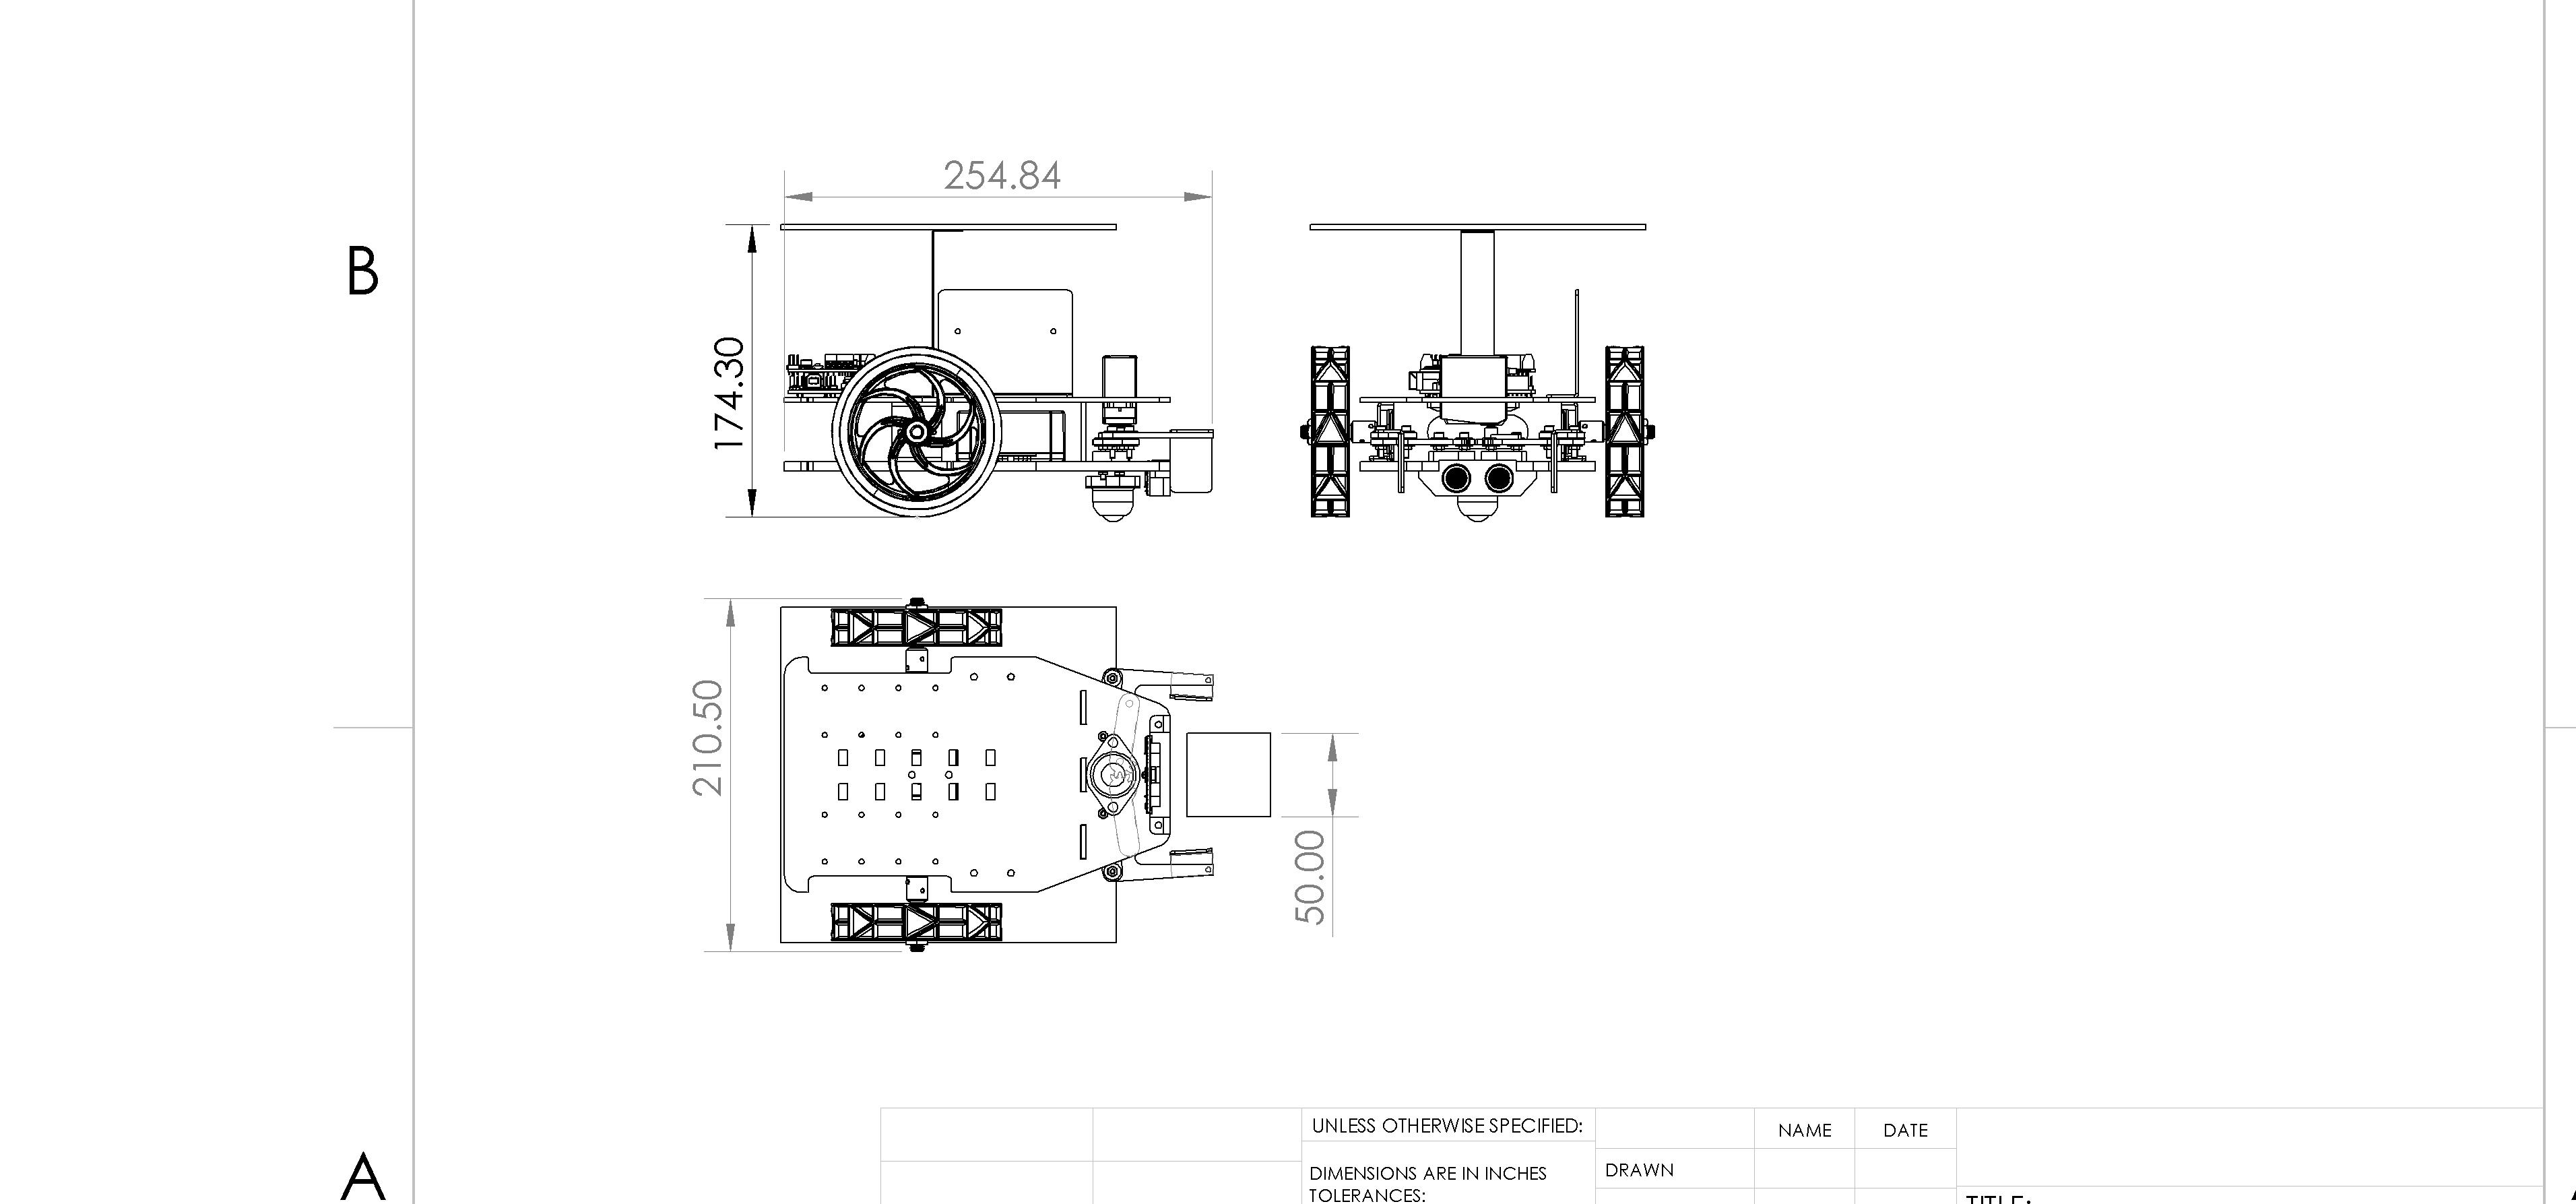
\includegraphics[width=0.8\textwidth]{assets/entire_model_drawing.jpg}
    \caption{Overall System Level Diagram}
    \label{fig:overall_sys}
\end{figure}

\end{document}
